\title{Deploying CouchDB Cluster}


\author{Ribka Rufael}
\orcid{}
\affiliation{%
  \institution{School of Informatics and Computing}
  \streetaddress{}
  \city{Bloomington} 
  \state{IN} 
  \postcode{47408}
  \country{USA}
}
\email{rrufael@iu.edu}



% The default list of authors is too long for headers}
\renewcommand{\shortauthors}{R. Rufael}


\begin{abstract}
  This project focuses on deployment of CouchDB Cluster using Ansible
  playbook on Ubuntu16.04 OS virtual machines on Chameleon Cloud by
  using Ansible script which is invoked by bash script. The deployment
  process provides the option of installing CouchDB version 2.1.1 in single node or
  cluster configuration. The deployment process also involves creation
  of database in CouchDB with different number of shards and replication. Part of this project
  also focuses on performing  benchmarking tests and analysis to asses the
  performance of CouchDB write, read and mapreduce tasks by variying
  the number of shards and replicas. 
\end{abstract}

\keywords{hid-sp18-703, CouchDB, Ansible, Chameleon Cloud}


\maketitle

\section{Introduction}

CouchDB~\cite{www-Couchdb} is a NoSQL database management system
under Apache. Data is stored as documents in CouchDB. In this project
CouchDB is deployed and configured on two Chameleon Cloud virtual machines using
Ansible playbook which is invoked through bash script. The two Chameleon
Cloud virtual machines have Ubuntu16.04 OS installed. The bash script
couchdbinstall.sh, by taking three command line parameters from user is
able to install and configure CouchDB in single or cluster
configuration.  This bash script also creates database with different
number of shards and replicas. 

Also in this project benchmarking tests were performed to find the
impact of number of shards and replicas on time taken for bulk
documents load into CouchDB, find documents operation and mapreduce
operation on documents in CouchDB. The bash script which is used to run the
benchmarking tests is DatasetBulkLoadReadCouchDB.sh.  The dataset which
was used for benchmarking tests on CouchDB is the wine quality dataset
from UCI Machine Learning Repository~\cite{www-WineQuality}. The
graphs used for the analysis of the benchmarking process were plotted
using plotBenchmark.py python script which utilizes pandas and
matplotlib libraries.

\section{Ansible}
Ansible is a tool that help automate software deployments, system
configuration and continues deployment of applications. Automation
tasks are defined in Ansible Playbooks using YAML language. For
transportation, Ansible uses OpenSSH~\cite{www-Ansible}. 

For this project, Ansible was used to install CouchDB, configure
CouchDB in single node or cluster configuration and to create database
in CouchDB with different number of replicas and shards configurations on
Chameleon Cloud virtual machines.

\section{Chameleon Cloud}

The Chameleon project provides open and large scale platforms for
reaserchers. Chameleon project gets its funding from National Science
Foundation (NSF). Reaserchers will be able to investigate and come up
with solutions for problems in the areas of Software as a Service, Platforms as a
Service and vitual technologies. Both Bare metal and OpenStack Virtual
environments are available for researchers to use on Chameleon
project~\cite{www-Chameleon}. 

For this project, OpenStack virtual machines were used. Launching of
new  virtual machine instances, assigning IP addresses to instances,
assigning security groups and other virtual management tasks were done
through the OpenStack web user interface~\cite{www-ChameleonDoc}. 


\section{Python}

Python programing language was used in two parts of this project. One
of the Python scripts was used for  preparing the test dataset with proper JSON format
used in CouchDB benchmarking process. Also Python was used to develop
the script which is used in the analysis of the benchmark process outputs.

\section{CouchDB}

Apache CouchDB is an open source and NoSQL database system. In CouchDB
data is stored in documents. Documents in CouchDB have unique names and contain
metadata. The content of the document in CouchDB is in semi structured
JSON format. The fields in the document can be different data types and there is no size
limit. Some of the supported data types for the content of documents
in CouchDB are strings, numbers, arrays, boolean and JSON objects~\cite{www-Couchdb}. 

There is no locking mechanism in CouchDB when adding,
updating or deleting documents. If two applications are making an
update to the same document in CouchDB database, upon save the
application has to resolve the conflict before merging the new
changes. Also while adding, updating or deleting documents in couchDB,
if the process fails before finishing then nothing gets saved in the
document. The update process has to finish successfully in order to
save the changes to the document. Read, write, update and delete
operations to CouchDB documents are done through RESTful
APIs~\cite{www-Couchdb}. 

User can interact with CouchDB through Fauxton which is
an administration user interface~\cite{www-Couchdb}. User can also
interact with CouchDB using  comand line tool called curl. Curl is
used to make call to the RESTful APIs through the command
line~\cite{www-CouchdbCurl}. 


Multi-Version Concurrency Control (MVCC) is used as concurrency model
in CouchDB. CouchDB uses views to present structured data to users and
applications. Views are implemented in Javascript. Views in CouchDB
use mapreduce model and they are stored under the design
documents~\cite{www-Couchdb}.  

\subsection{Version}
The version of CouchDB used for this project is version 2.1.1 and this
is the current version at the time of writing this report.

\subsection{Architecture}
CouchDB 2.1.1 provides two setup configurations. These setup
configurations are single node and clustered configurations. As the
name suggests, CouchDB in single node configuration runs on a single
node. Whereas in clustered configuration CouchDB runs on multiple
nodes or servers~\cite{www-Couchdb, www-CouchdbOverview}.

\subsection{Cluster Shards and Replicas}

Shards are partions of database table which are split by
rows~\cite{www-WikiShard}. The number of copies of each document in
CouchDB database is called replica~\cite{www-CouchdbTheory}. When
creating databases in CouchDB cluster, user can provide the number of
shards and replicas. If the user does not provide the number of shards
and replicas, CouchDB sets the default values of 8 shards and 3
replicas. Having the number of replicas
greater than one increases the failure resistance of the cluster. In
scenarios where we have multiple replicas and one of the replicas fail
then user can still perform read and write operations on documents
without any disruption~\cite{www-CouchdbTheory}.

\subsection{Security}
The ports that are used by CouchDB cluster are 5984 and 5986. Port
4369 is used by Erlang to identify the nodes in CouchDB cluster. Also
ports 9100-9200 for Erlang on different virtual machines to communicate to each
other. These ports should be opened to accept TCP protocol for all the
servers or virtual machines that are in the
cluster~\cite{www-CouchdbSetup}. 

In the deployment for this project, security group rules were
created in Chameleon Cloud which opened inbound TCP protocol for ports
5984, 5986 and 9100-9200.


\section{Deployment}
The deployment of CouchDB  was done through an automated Ansible
playbook which is invoked by bash script.
\subsection{Resource}
Table \ref{t:resource-specification} provides the specification for
the Chameleon Cloud Virtual Machines used in this project.

\begin{table}[]
\centering
\caption{Resource Specification}
\label{t:resource-specification}
\begin{tabular}{|l|l|l|l|l|l|}
\hline
\textbf{Instance} & \textbf{Image}       & \textbf{Size} & \textbf{RAM} & \textbf{VCPUs} & \textbf{Disk} \\ \hline
Node1             & Ubuntu16.04-20180205 & m1.medium     & 4GB          & 2              & 40GB          \\ \hline
Node2             & Ubuntu16.04-20180205 & m1.medium     & 4GB          & 2              & 40GB          \\ \hline
\end{tabular}
\end{table}

Before starting the deployment of CouchDB, user have to perform the
following preparation steps.
\begin{enumerate}
  \item Start two Instances in Chameleon Cloud with the specification
    in Table 1~\ref{t:resource-specification}
   \item  Allocate floating IPs to the instance created
    \item Add  security rules as mentioned under Security section
      of this report to the two instances 
    \item  User has to manually insert the IP addresses by modifying
      inventory.txt file which is found under project-code
      /couchdbansible directory. There are two hosts 
      defined under inventory.txt. One of the IP addresses
      goes under \verb|[couchdb_Coordination_host]| section of inventory.txt
      and the second IP address goes under \verb|[couchdb_hosts]|.
\end{enumerate}

\subsection{couchdbinstall.sh}

The bash script couchdbinstall.sh, takes three command line inputs
from the user. First parameter tells the script whether to install
CouchDB in single node or cluster configuration. The second input
represents the
number of replicas. The third input is the number of shards. An
example command looks like `./couchdbinstall.sh true 3 8` which
deploys CouchDB in cluster configuration and creates a database with 3
replicas and 8 shards.

The Ansible script that deploys CouchDB and it's dependencies are run
within couchdbinstall.sh. This script also creates CSV file which
contains information about cluster setup, number of replicas, number
of shards and the time it took for couchDB install.

\subsection{Ansible Scripts}
All Ansible scripts reside under /project-code/couchdbansible
directory. 
\begin{enumerate}
  \item playbook.yml- defines the hosts on which CouchDB will be
    installed and the role name. This file along with inventory.txt is
    needed when runing Ansible playbook.

  \item main.yml-this file which is found under /roles/couchdb/tasks
    directory and this where all the installation tasks are
    defined. Some of the tasks defined are installation of Python
    pandas library since the virtual machines in Chameleon did not have pandas
    installed, installation of CouchDB 2.1.1 and all it's dependencies
    and database creation after the installation of CouchDB.

  \item vmargs.j2- under /roles/couchdb/templates directory, template
    file that defines the CouchDB node names with the correct IP addresses.
\end{enumerate}

\subsection{Deploy Time}
The time taken for deployment of CouchDB on two Chameleon VMs was recorded for different
scenarios. As it can be seen in table~\ref{t:CouchDB-DeployTime},
CouchDB was installed in single node configuration/cluster configuration and different
number of replicas and shards. The first scenario which is basic installation of CouchDB
in single node configuration and no replicas and shards took 54 seconds
amount of time to finish. The sceond scenario, installation of CouchDB
in cluser configuration with two nodes configuration, 3 replicas and
8 shards took 52 seconds. The third scenario, installation of CouchDB
in cluser configuration with two nodes configuration, 4 replicas and
12 shards took 53 seconds. 

\begin{table}[]
\centering
\caption{CouchDB Deploy Time}
\label{t:CouchDB-DeployTime}
\begin{tabular}{|l|l|l|l|l|}
\hline
  & \textbf{Cluster\_Setup} & \textbf{replica\_val} & \textbf{shard\_val} & \textbf{Install time in seconds} \\ \hline
1 & False                   & 1                     & 1                   & 54                               \\ \hline
2 & True                    & 3                     & 8                   & 52                               \\ \hline
4 & True                    & 4                     & 12                  & 53                               \\ \hline
\end{tabular}
\end{table}

\section{Benchmark Results}
\subsection{Dataset}
The dataset that was used for the benchmarking process for this
project is the white vinho verde varient of Portuguese wine sample
from UCI Machine Learning Repository. The size of the dataset used for
this project winequality-white.csv is 258KB. The dataset was in CSV file
format and contains twelve different attributes related to wine such
as fixed acidity,pH, alcohol and quality~\cite{www-WineQuality}. 

Since CouchDB bulk load process only accepts file in proper JSON
format, \verb|csv_to_json.py| python script was used to download the
white wine dataset (winequality-white.csv) directly from UCI Machine
Learning Repository and convert the CSV file into JSON format by utilizing
pandas and urllib Python libraries. After converting into CouchDB
compatible JSON format the dataset size was 1.1MB.

\subsection{DatasetBulkLoadReadCouchDB.sh}
This is the script when executed, loads the JSON wine sample dataset
into CouchDB, performs simple read operation on the wine sample
dataset in CouchDB and mapreduce on the wine sample
dataset in CouchDB. It also measures the time taken for each operation.

\begin{enumerate}
  \item The first thing this script does is, it copies
    \verb|csv_to_json.py| Python script to the remote VM and executes
    this script inorder to generate the JSON wine dataset.
  \item CouchDB has \verb|/{db}/_bulk_docs| endpoint that is used to
    create multiple documents with singe POST
    request~\cite{www-CouchdbBulkApi}. DatasetBulkLoadReadCouchDB.sh
    loads JSON wine dataset into `test` database in CouchDB  using
    this POST call through curl command. Then measures the time taken
    to finish the bulk documents load operation.

  \item DatasetBulkLoadReadCouchDB.sh performs find document operation
    to find documents from wine dataset which have quality greater
    than 3. Then measures the time taken to finish this find
    operation. The find operation is accomplished by making POST call
    to \verb|/{db}/_find| endpoint which returns documents that meet
    query criteria~\cite{www-CouchdbFind}. 

  \item We wrote mapreduce function mapreducefun.js, which returns
    total number of rows from wine dataset which have quality greater than 3. This mapreduce
    function was uploaded to CouchDB design document to create view and GET call to
    \verb|/db/_design/design-doc/_view/view-name| was
    made~\cite{www-CouchdbView}. DatasetBulkLoadReadCouchDB.sh
    executes this mapreduce function on wine dataset in CouchDB and
    measures the time taken to finish execution of mapreduce.
  \item The final step in DatasetBulkLoadReadCouchDB.sh is to gather
    all the time durations from these mentioned operations and save
    into CSV file under /CouchDBBenchmark directory.

\end{enumerate}

\subsection{Benchmark Result Analysis}
There were two aims of the benchmarking process for this project. One
of the aims of the benchmarking process was to find the impact of
number of shards on bulk documents load into CouchDB, find documents
operation and map reduce on documents in CouchDB. The second aim of
the process was to find the impact of number of replicas on bulk
documents load into CouchDB, find documents operation and map reduce
on documents in CouchDB. 

Tests involving different combination of number of replicas and shards
were performed and the results were captured in CSV files. All these
CSV files were combined into one CSV file named CouchDBfinal.csv under
/project-code/CouchDBBenchmark directory by running
CombineBenchmark.sh bash script. Finally, we developed
plotBenchmark.py python script that takes combined CSV files and plots
the graphs which will be discussed in the sections to follow. For the
purpose of reproducing the graphs in this project in the future, CSV file used
CouchDBfinal.csv is saved under project-artifact directory. 

To asses the impact of number of shards, number of replicas was set to a
constant value of 3 and tests were performed. The number of shards
used were 1,2,4,6,10 and 12. To asses the impact of replicas, number
of shards was set to a constant value of 1 and tests were
performed. The number of replicas used were 1,2,3,4 and 6.



\subsubsection{Number of Shards Impact on Bulk Load}


Figure~\ref{f:shard-bulk} depicts the the impact of number of shards
on bulk load documents to couchDB time in seconds. As it can be seen
in the graph, it took 3 seconds to bulk load documents in couchDB when
the number of shards was one. For number of shards starting from
two onwards, the bulk load time decreased to a value of 2 seconds and remained
constant. It took less time for bulk load documents when the number of
shards increased from one to two.

\begin{figure}[!ht]
  \centering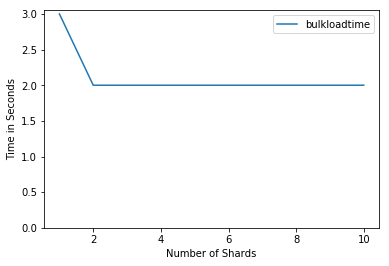
\includegraphics[width=\columnwidth]{../images/ShardsBulkLoad.png}
  \caption{Number of Shards vs Bulk Load Time in seconds }\label{f:shard-bulk}
\end{figure}



\subsubsection{Number of Shards Impact on Document Find}


Figure~\ref{f:shard-find} shows the impact of number of shards on find
documents on CouchDB time in seconds. There was not any performace
improvement of the time it took to find documents in CouchDB  by
changing the value of the number of shards. As the it can be seen in
~\ref{f:shard-find} the time for find documents remained at 1 second
regardless of changing the the number of shards.

\begin{figure}[!ht]
  \centering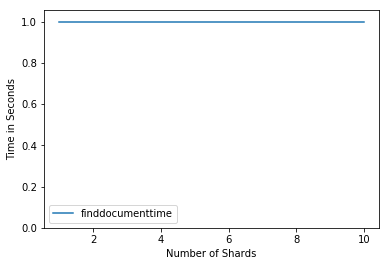
\includegraphics[width=\columnwidth]{../images/ShardsFindDoc.png}
  \caption{Number of Shards vs Find Document Time in seconds }\label{f:shard-find}
\end{figure}

\subsubsection{Number of Shards Impact on MapReduce}


Figure~\ref{f:shard-mapreduce} shows the impact of number of shards on
mapreduce process on CouchDB time in seconds. When the number of shards was one, it took 4 seconds to finish
the mapreduce operation. It took 3 seconds to finish
the mapreduce operation when the values of shards were between two and
six. There was a performance
improvement for time taken for performing mapreduce operations for shards two, four and six.  The time duration started to
go up after increasing the number of shards to eight and above. There
is no performance improvement on the time for mapreduce operations by
increasing the number of shards greater than six.

\begin{figure}[!ht]
  \centering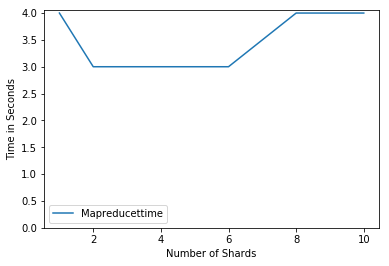
\includegraphics[width=\columnwidth]{../images/ShardsMapReduce.png}
  \caption{Number of Shards vs Mapreduce Time in seconds }\label{f:shard-mapreduce}
\end{figure}

\subsubsection{Number of Replicas Impact on Bulk Load}


Figure~\ref{f:replica-bulk} depicts the the impact of number of replicas
on bulk load documents to couchDB time in seconds. As it can be seen
in the graph, it took 3 seconds to bulk load documents in couchDB when
the number of replicas was one. There was a decrease in time
taken when the number of replicas was two. Then as the value of
replicas increased to three and above the time it took for documents
bulk load increased to 3 seconds and remained the same. The increase
of time as the number of replicas increases is expected because the
documents have to be copied the same number of times as the number of
replicas. 


\begin{figure}[!ht]
  \centering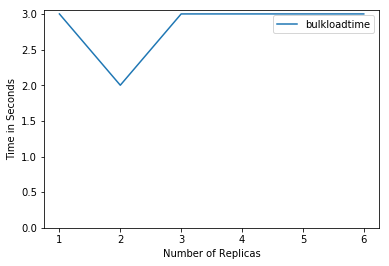
\includegraphics[width=\columnwidth]{../images/ReplicasBulkLoad.png}
  \caption{Number of Replicas vs Bulk Load Time in seconds }\label{f:replica-bulk}
\end{figure}

\subsubsection{Number of Replicas Impact on Document Find}


Figure~\ref{f:replica-find} shows the impact of number of replicas on find
documents on CouchDB time in seconds. There was not any performace
improvement of the time it took to find documents in CouchDB  by
changing the value of the number of replicas. As the it can be seen in
~\ref{f:replica-find} the time for find documents remained at 1 second
regardless of changing the the number of replicas.

\begin{figure}[!ht]
  \centering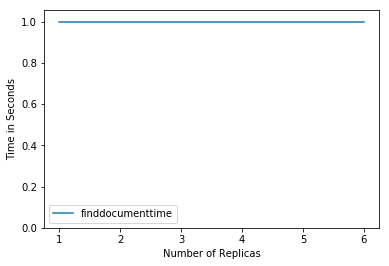
\includegraphics[width=\columnwidth]{../images/ReplicasFindDoc.png}
  \caption{Number of Replicas vs Find Document Time in seconds }\label{f:replica-find}
\end{figure}

\subsubsection{Number of Replicas Impact on MapReduce}


Figure~\ref{f:replica-mapreduce} shows the impact of number of replicas on
mapreduce process on CouchDB time in seconds. The time it took for
mapreduce operation was 3 seconds for one, two and six replicas. For
replicas three and four mapreduce operation took 4 seconds. The
variations in time could be related to network speeds at the time of
executing the tests as these API requests are made through network. 

\begin{figure}[!ht]
  \centering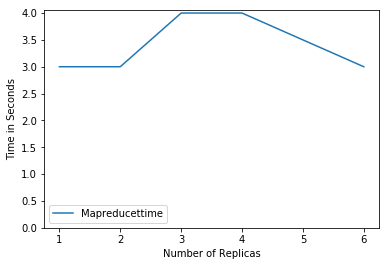
\includegraphics[width=\columnwidth]{../images/ReplicasMapReduce.png}
  \caption{Number of Replicas vs Mapreduce Time in seconds }\label{f:replica-mapreduce}
\end{figure}

\section{Conclusion}
This project succesfully deployed and configured CouchDB  on two virtual machines
on Chameleon cloud using Ansible playbook which is invoked through
bash script. The bash script also allowed CouchDB to be configured in
single node or cluster configuration and created database with
different number of shards and replicas. Although for the purpose of
this project only two virtual machines on Chameleon cloud were used,
the Ansible script will be able to support installation of CouchDB to more
than two virtual machines by providing more host IP addresses under
inventory.txt for Ansible.

Analysis of benchmarking tests showed that there was not any performace
improvement of the time it took to find documents in CouchDB  by
changing the value of the number of shards or replicas. For number
shards between two to six, there was a performance improvement for
time taken for performing mapreduce operations. In general, mapreduce
took more time than find documents operation for different number
shards and replicas, which could be the result of mapreduce using
JavaScript query server for map and reduce operations.


\section*{Acknowledgements}

The author would like to thank Professor Gregor von Laszewski and
associate instructors for their help and guidance.


\bibliographystyle{ACM-Reference-Format}
\bibliography{report} 
\appendix
\section{Project Code Execution}
All the codes for this project are under project-code
directory. There are three directories under project-code.
\begin{itemize}
  \item CouchDBBenchmark which contains CSV files from deployment and
    benchmarking processes.  
  \item couchdbansible which contains Ansible scripts
  \item logs which contains console output logs
\end{itemize}

 Before starting the deployment of CouchDB, user have to
perform the following preparation steps.
\begin{enumerate}
  \item Start two Instances in Chameleon Cloud with the specification
    in Table 1~\ref{t:resource-specification}
   \item  Allocate floating IPs to the instance created
    \item Add  security rules as mentioned under Security section
      of this report to the two instances 
    \item  User has to manually insert the IP addresses by modifying
      inventory.txt file which is found under project-code
      /couchdbansible directory. There are two hosts 
      defined under inventory.txt. One of the IP addresses
      goes under \verb|[couchdb_Coordination_host]| section of inventory.txt
      and the second IP address goes under \verb|[couchdb_hosts]|.
\end{enumerate}

\subsection{Deploy CouchDB}
To deploy CouchDB, on command prompt cd to project-code/ directory and run
couchdbinstall.sh as providing three parameters. 
\begin{enumerate}
  \item First parameter takes true or false to indicate whether to
    install CouchDB in single node or cluster
    \item Second parameter is an integer number for the value of
      replica
      \item Third parameter is an integer number for the value of
      shard
\end{enumerate}
An example command


./couchdbinstall.sh true 3 8 

\subsection{Benchmark Tests}
To run benchmark tests, on command prompt cd to project-code/ directory and run
./BulkLoadReadCouchDB.sh
This script performs different benchmark tests and saves all the time
durations into CSV file name starting with \verb|benchmark_| under
CouchDBBenchmark directory.

\subsection{Combining CSV files}
To combine all CSV files from Benchmarking tests into one file named CouchDBfinal.csv run
./CombineBenchmark.sh 


A copy of this file is also saved under project-artifact if needed in
the future to reproduce the graphs in this project

\subsection{Plotting graphs for Benchmark Tests}
To Plot the graphs for benchmarking analysis run the 
plotBenchmark.py script from command line as follows

python plotBenchmark.py











